U ovom poglavlju upisani su algoritmi koji su potrebni za konstruranje i korištenje FM-indeksa u svrhu prebrojavanja broja ponavljanja podniza unutar zadanog niza nad kojim je konstruiran FM-indeks. Opisani su algoritmi Burrows-Wheeler transformacije, wavelet stabla i RRR strukture.


\section{Burrows-Wheeler transformacija}
Burrows-Wheeler transformacija (skraćeno BWT) \cite{bwt1}, služi za kompresiju tekstualnog niza na osnovi pronalaska ponavljajućih uzoraka unutar njega. Ova transformacija je reverzibilna i ne iziskuje pohranu dodatnih podataka za rekonstrukciju originalnog niza. Osim ovoga, prilikom BWT transformacije, ni jedan znak originalnog niza se ne mijenja. Dodatna prednost je činjenica da se za transformaciju (osim dodavanja znaka \$) ne proširuje ulazna abeceda. Ukoliko ulazni niz sadrži više jednakih podnizova, velika je vjerojatnost da će transformirani niz sadržavati uzastopne nizove jednakih znakova, što kasnije uvelike pogoduje njegovom komprimiranju.

\subsection{Algoritam transformacije}
Algoritam transformacije provodi se u 4 koraka:

\begin{enumerate}
  \item Na kraj teksta postavlja se znak \$ koji označava kraj te je, leksikografski gledano, najmanji znak ulazne abecede.
  \item Stvara se matrica svih različitih cikličkih pomaka niza dobivenog nakon 1. koraka.
  \item Matrica iz koraka 2 se sortira u leksikografskom poretku.
  \item Dobivena transformacija isčitava se iz poslijednjeg stupca matrice dobivene u koraku 3.

\end{enumerate}

Tijek algoritma za riječ "banana" prikazan je na slici \ref{bwt1}. Vidi se kako je BWT transformacija te riječi jednaka annb\$aa. 


\begin{figure}[H]
\centering
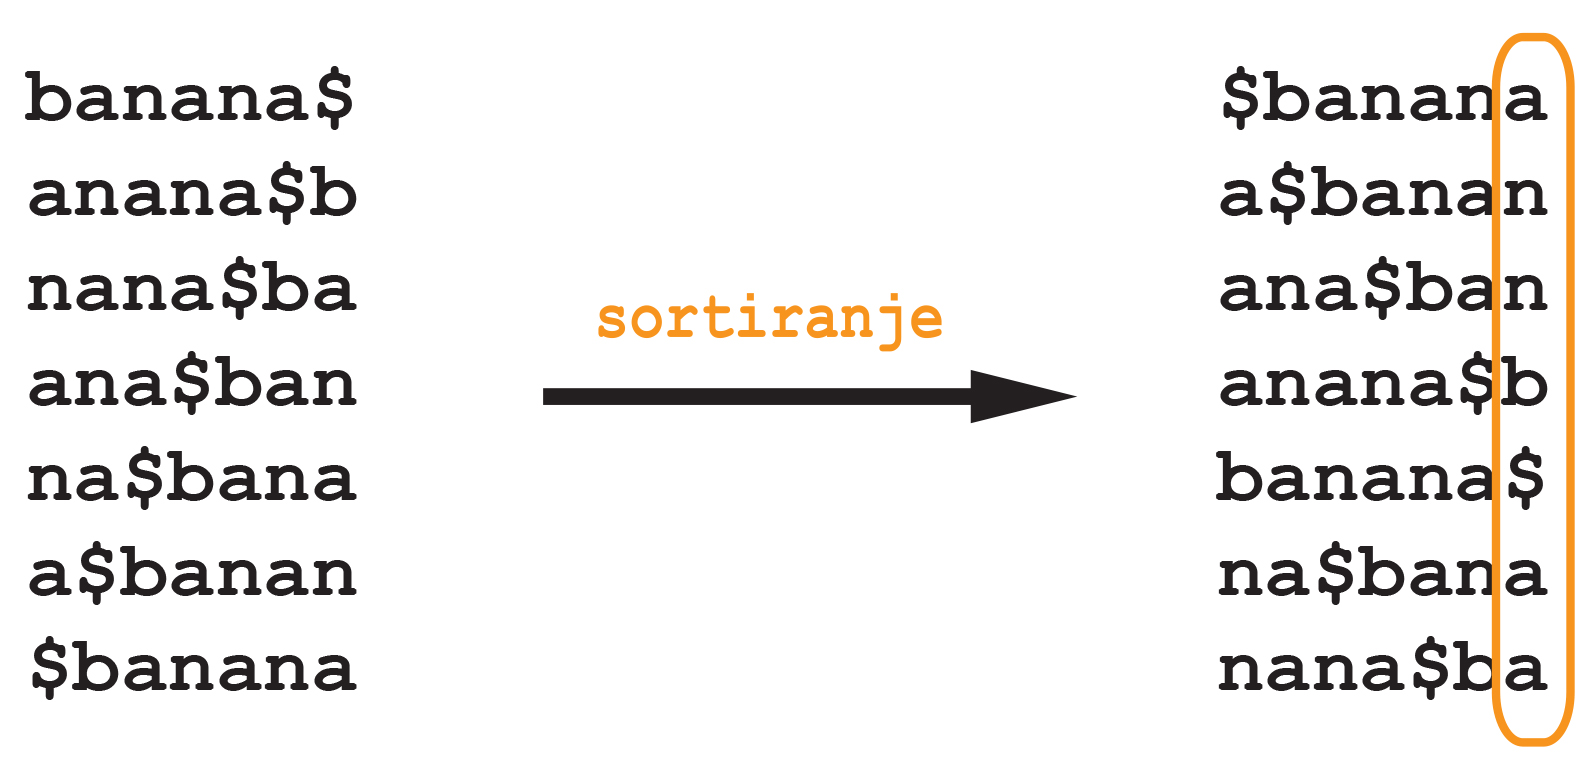
\includegraphics[scale=0.2]{./pictures/bwt.jpg}
\caption{Ispunjene vrijednosti u poljima BS i SBS}\label{bwt1}
\end{figure}

\subsection{Rekonstrukcija originalnog teksta iz BWT transformacije}
Matrica dobivena u 3. koraku algoritma poslužiti će za rekonstrukciju originalnog teksta iz dane BWT transformacije. Naime, ta matrica ima svojstvo da u svakom njenom retku, zadnji znak prethodi prvom znaku u istom retku matrice u originalnom tekstu. To znači, da je za rekonstrukciju izvornog teksta dovoljan samo prvi i zadnji stupac te matrice. Budući da je poznatno da tu matricu čine sve permutacije ulaznog niza i to sortiranog, jednostavno se može rekonstruirati prvi stupac - jednostavno se uzmu i sortiraju svi znakovi danog transformiranog niza. Budući da znamo da je posljednji znak u nizu znak \$, lako je iz prvog i zadnjeg stupca matrice rekonstruirati originalni niz. Na slici \ref{bwt2} prikazan je postupak rekonstrukcije originalnog niza (sivi brojevi na desnoj strani označavaju broj koraka).

\begin{figure}[H]
\centering
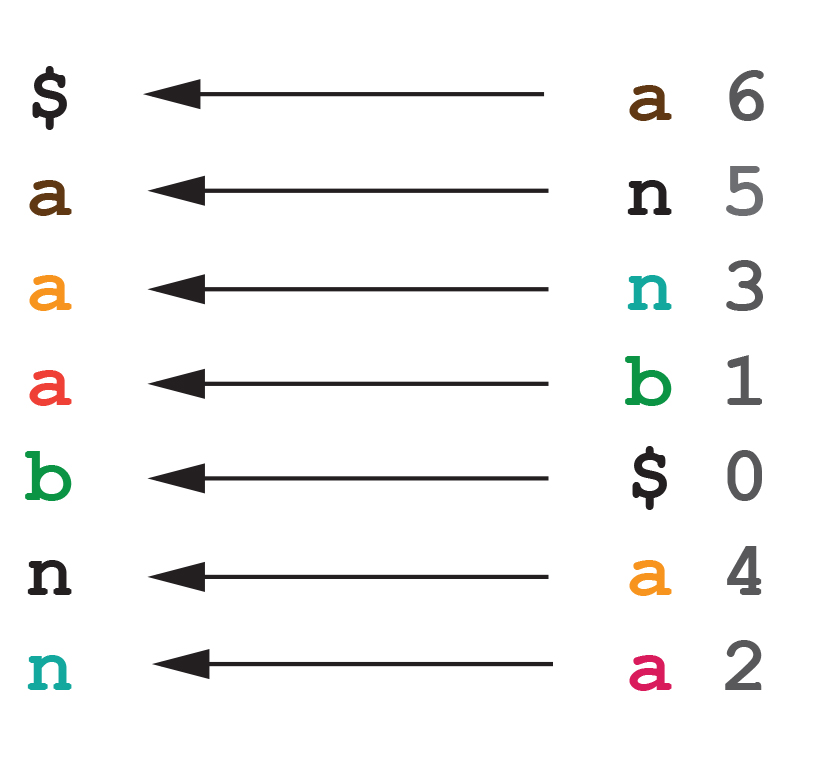
\includegraphics[scale=0.2]{./pictures/reverseBWT.jpg}
\caption{Ispunjene vrijednosti u poljima BS i SBS}\label{bwt2}
\end{figure}

\subsection{Konstrukcija BWT-a}
Iako je sam algoritam izgradnje BWT transformacije veoma jednostavan, nažalost nije i efikasan. Za poveće tekstove je jednostavno nemoguće napraviti sve njihove rotacije i onda ih sortirati, jer bi memorijsko zauzeće bilo preveliko. Iz tog razloga potrebno je koristiti algoritme koji BWT transformaciju mogu obaviti memorijski i vremenski efikasno. U nastavku ćemo pogledati dva takva algoritma te vidjeti koje su njihove prednosti i nedostatci.

\subsection{Multikey quicksort}
Prvo ćemo proučiti jedan tip algoritma za sortiranje koji se temelji na quick sort algoritmu predloženom u \cite{mkqs}. Prednost ovog algoritma jest u tome da može sortirati sve rotacije jednog niza koristeći samo osnovni niz i dodatno polje pokazivača na taj niz. Na taj način nije potrebno raditi sve rotacije ulaznog niza. Algoritam u svojoj osnovi spaja quick sort i radix sort. Osnovni koraci algoritma prikazani su na slici \ref{mkqs}  Prvo se nasumično odabere jedan niz, a prvi element toga niza je pivot. Odabrani niz se nakon toga zamijeni s prvim nizom. Sada djelomično sortiramo sve nizove tako da se nizovi koji počinju s elementom koji je jednak pivotu pozicioniraju na početak ili kraj niza, dok se ostali nizovi poredaju tako da tako da se u prvom dijelu nalaze svi nizovi koji započinju elementom koji je manji od pivota (u primjeru na slici je to niz koji započinje s "\$"), dok se u drugom dijelu nalaze nizovii koji započinju s elementom koji je veći od pivotna (u primjeru su to nizovi koji započinju s "b" i "n"). Idući korak jest da se svi nizovi koji započinju elementom koji je iznosom jednak pivotu premjeste u sredinu i to tako da se nizovi koji započinju s manjim elementom nalaze ispred njih, a nizovi koji započinju s većim elementom iza njih.  Sada su nizovi efektivno podijeljeni u tri dijela, prvi dio koji sadrži nizove koji započinje elementom koji je manji od pivora, drugi dio koji čine nizovi koji počinje elementima koji su jednaki pivotu i treći dio koji sačinjavaju nizovi  koji započinju elementom koji je veći od pivota. Sada kada imamo ovu podjelu, svaki od ta tri dijela je potpuno neovisan o drugima i svi se mogu nezavisno sortirati (ovdje je očita i jedna prednost ovog postupka koju ćemo kasnije naglasiti). Sada prvu i treću grupu nizova sortiramo na isti način kao što smo sortirali sve nizove. Drugu grupu ćemo sortirati na isti način, jedina će razlika biti da ćemo sada sortirati po drugom znaku tih nizova (jer je očito da su sortirani po prvom znaku), no ostatak algoritma je u potpunosti jednak. Algoritam se nastavlja dok svi nizovi nisu u potpunosti međusobno sortirani.


\begin{figure}[h]
   \centering
       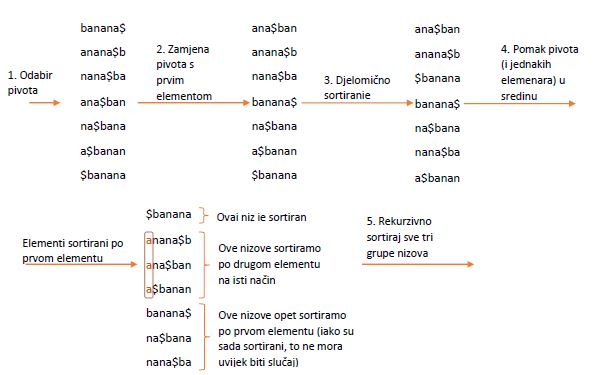
\includegraphics[width=\textwidth]{./pictures/MKQS.jpg}
 \caption{Multikey quicksort algoritam}
 \label{fig:Test}
\end{figure}

Bitno je za napomenuti da je zbog ilustracije rad algoritam prikazan na nezavisnim nizovima (kao da smo prvo napravili sve rotacije osnovnog niza i onda njih sortirali). Naravno u implementaciji to nije tako napravljeno, već postoji niz brojeva koji predstavljaju pokazivače (odnosno indekse pošto pokazivači ne postoje u programskom jeziku Java) na elemente ulaznog polja. Onda umjesto da se zamjenjuju čitavi nizovi jednostavno se zamijene pokazivači u tom polju.

Prednost ovog postupka su prije svega njegova jednostavnost. Sam algoritam je veoma intuitivan i nije ga teško razumjeti. Druga, mnogo očitija prednost jest mogućnost paralelizacije ovog algoritma. Kako je ranije navedeno, nizovi su na kraju podijeljeni u tri nezavisne grupe, od kojih se svaka sortira nezavisno. To znaći da bi teoretski svaku ovu grupu mogli sortirati međusobno paralelno. Nažalost zbog veoma loše implementacije paralelnih mehanizama u programskom jeziku Javi , ovo ipak nije napravljeno. No kada bi implementacija bila napravljena u nekom programskom jeziku koji je više specijaliziran za paralelizaciju to bi bilo dobro napraviti. Najveći nedostataci ovog postupka su svakako nešto veća složenost naspram konstrukcije BWT-a korištenjem sufiksnog polja, ta također rekurzivna priroda algoritma koja zahtijeva puno rekurzivnih poziva i iz tog razloga također i alokaciju veće količine memorije za stog.

Iako se ovdje radi o veoma zanimljivom algoritmu (algoritmu koji nije naravno primjenjiv samo na pronalazak BWT transformacije), nažalost pokazao se je kao prespor u usporedbi s izračunavanjem BWT transformacije korištenjem sufiksnog polja.

\subsection{Konstrukcija sufiksnog polja}
Sufiksno polje jest jednostavna stuktura podataka koje je sastavljena od niza cijelih brojeva koji sadrže početna mjesta abecedno poredanih sufiksa nekog niza. Dobra stvar kod sufiksnog polja jest da se iz njega može izračunati BWT transformacija u linearnom vremenu. Još veća prednost ovakvog postupka jest da se sufiksno polje isto tako može konstruirati u linearnom vremenu. Iako postoje mnogi algoritmi za konstrukciju sufiksnih polja, u ovoj implementaciji iskorišten je algoritam koji je predložen u \cite{sais1} i \cite{sais2}. 

Prije nego što se krene na objašnavanje samog algoritma potrebno je uvesti određenu terminologiju koju ćemo koristiti za objašnjenje postupaka ovog algoritma. Ulazni niz znakova ćemo označiti sa $S$. Neka je ulazni niz znakova duljine $n$, i neka je oznaka indeksiranja jednog elementa $S[i]$ pri ćemu je $i \in [0,n-1]$. Posljednja stvar koju je bitno napomenuti jest da znakovni niz mora obavezno završavati znakom koji je strogo manji od svih znakova u ostatku niza.  Definirat ćemo dvije različite vrste znakova, L-znakove i S-znakove. S-znak je onaj znak koji je manji od znaka koji dolazi neposredno iza njega (odnosno formalnije, ako gledamo i-ti znak onda mora vrijediti $S[i]<S[i+1]$) ili je jednak znaku koji se nalazi desno od njega i taj znak je S-znak (formalnije $S[i]=S[i+1]$ i $S[i+1]$ je L-znak). L-znak je onaj znak za koji vrijedi da je veći od znaka koji se nalazi desno od tog znaka (odnosno formalnije, ako gledamo i-ti znak onda mora vrijediti $S[i]<S[i+1]$) ili je jednak znaku koji se nalazi desno od njega i taj znak je L-znak (formalnije $S[i]=S[i+1]$ i $S[i+1]$ je L-znak). Iznimka od ovog pravila jest zadnji znak koji će uvijek biti definiran kao S-znak. Ovaj koncept možemo proširiti i na sufikse, pa reći da je S-sufiks sufiks koji počinje S-znakom i L-sufiks sufiks koji počinje L-znakom. Uvest ćemo još pojam LMS-znak i LMS-podniz. LMS-znak je S-znak kojemu se na lijevom mjestu nalazi L-znak, odnosno vrijedi $S[i]$ je S-znak i $S[i-1]$ je L-znak. LMS-podniz je niz koji započinje LMS-znakom i završava LMS-znakom, te se u njemu ne nalaze drugi LMS-znakovi. Primjer jednog ovako označenog niza može se vidjeti na slici \ref{fig:oznake}.

\begin{figure}[h]
   \centering
       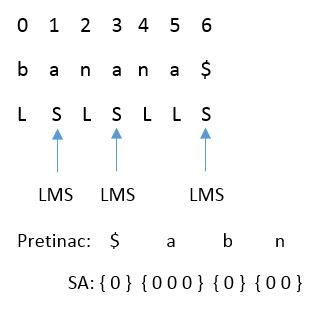
\includegraphics{./pictures/charactertypes.jpg}
 \caption{Oznake znakova u jednom nizu}
 \label{fig:oznake}
\end{figure}

Sada kada su uvedene osnovne oznake, možemo pojasniti samo ideju algoritma. Osnovna ideja algoritma predložena je već u \cite{ka}. U svojoj osnovnoj inačici, algoritam se je zasnovao na svojstvu da ako znamo poredak svih S-sufiksa ona možemo odrediti i poredak svih L-sufiksa. Nažalost, problem je ostao u tome kako zapravo efikasno sortirati S-sufikse. U tom radu je predložen način kako bi se to moglo riješiti korištenjem S-udaljenosti, što je opet zahtjevalo dodatnog memorijskog prostora. Ta ideja je razrađena i poboljšana te je konačno predložen novi algoritam u [nang] koji se zasniva na istoj ideji, ali uvodi neke promjene koje su rezultirale mnogo boljim ponašanjem ovog algoritma. Prvo bitno poboljšanje koje je uvedeno jest da se umjesto sortiranja S-sufiksa mogu sortirati LMS-sufiksi, koji su sasvim dovoljni kako bi se odredio poredak L-sufiksa, pomoću kojih se konačno može odrediti poredak S-sufiksa. Kako su LMS-sufiksi obično dulji, to znaći kako ćemo vjerojatno imati manji broj takvih sufiksa koje moramo sortirati nego bi to bio slučaj da sortiramo sve S-sufikse (u najgorem slučaju broj LMS-sufiksa je polovica duljine ulaznog niza). Drugo veoma zanimljivo poboljšanje jest da se za sortiranje tih LMS-sufiksa ne mora koristiti nikakav posebni algoritam za sortiranje nego se može koristiti isti postupak kao i kod sortiranja L-znakova i S-znakova. U nastavku ćemo pogledati detaljnije korake ovog algoritma. 

Prvo je potrebno svim znakovima odrediti jesu li to S-znakovi, L-znakovi ili LMS-znakovi. Nakon tog koraka slijedi postupak induciranog sortiranja. Definirajmo prvo inducirano sortiranje. To je postupak kojim ćemo iz LMS-sufiksa inducirati poredak L-sufiksa i potom S-sufiksa. Ovo je zapravo centralni i najvažniji dio algoritma. Za rad ovog algoritma potrebno nam je nekoliko struktura: ulazni niz, sufiksno polje, niz sa oznakama tipova znakova i pokazivaći na pretince. Sve strukture su već ranije spomenute i poznate, osim pokazivaća na pretince. Pretince ćemo zapravo definirati kao područja u nizu u kojima se nalaze sufiksi koji počinju s  istim početnim znakom. Broj pretinaca će dakle biti jednak veličini abecede (originalne abecede proširene s dodatnim znakom koji je manji od svih ostalih). Kada imamo sve te strukture možemo provesti postupak induciranog sortiranja. Postupak induciranog sortiranja se provodi kroz tri koraka opisanih u nastavku.

Prije početka prvog koraka pretpostavimo da svi pokazivaći na pretince pokazuju na krajeve tih pretinaca, i neka su vrijednosti elemenata sufiksnog polja inicijalno postavljene na vrijednost 0. Prvi korak se sastoji od toga da prođemo kroz niz i da sve LMS-znakove stavimo u odgovarajući pretinac (smjer prolaska kroz niz je u potpunosti nebitan, može se prolaziti od početka ili od kraja niza). Kada stavimo LMS-znak u odgovarajući pretinac potrebno je pokazivač na taj pretinac smanjiti tako da pokazuje ne iduće prazno mjesto. Ovaj korak algoritma detaljno je prikazan na slici \ref{fig:sais1}

\begin{figure}[H]
   \centering
       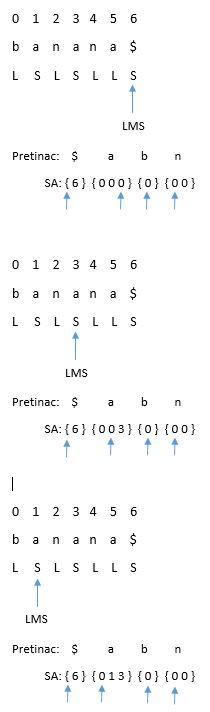
\includegraphics{./pictures/SAISstep1.jpg}
 \caption{Prvi korak u induciranom sortiranju}
 \label{fig:sais1}
\end{figure}

Prije početka drugog koraka potrebno je pokazivače postaviti na početke svih pretinaca. Drugi korak algoritma jest induciranje L-znakova. U ovom koraku prolazimo kroz sufiksno polje s lijeva na desno i za svaki element koji je veći od 0, dakle za elemente za koje vrijedi $SA[i]>0$. Svaki taj  element zapravo predstavlja indeks nekog znaka u ulaznom nizu. Za svaki element iz sufiksnog polja ispitat ćemo da li je znak iz ulaznog niza koji se nalazi na poziciji koja je određena vrijednošću trenutnog elementa sufiksnog polja umanjenoj za jedan L-znak. Mnogo jednostavnije rečeno  ispitujemo da li je znak $S[SA[i]]$ L-znak, pri ćemu je $i$ index elementa sufiksnog polja na kojem se trenutno nalazimo. Ukoliko je taj znak L-znak, onda u pretinac koji predstavlja taj znak stavimo njegov indeks i uvećamo pokazivač na taj pretinac. 

\begin{figure}[H]
   \centering
       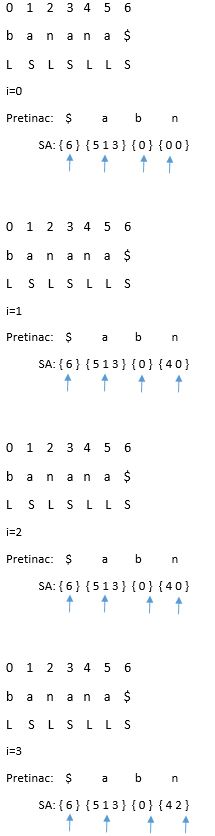
\includegraphics{./pictures/SAISstep2.jpg}
 \caption{Prvi korak u induciranom sortiranju}
 \label{fig:sais2}
\end{figure}

Prije početka treće i posljednje faze induciranog sortiranja moramo pokazivače postaviti na kraj pretinaca. Treći dio induciranog sortiranja je veoma sličanan drugom koraku. Kroz sufiksno polje se ovaj puta prolazi od kraja prema početku. Opet izostavljamo elemente koji su jednaki 0.  Za svaki element iz sufiksnog polja ispitat ćemo da li je znak iz ulaznog niza, koji se nalazi na poziciji koja je određena vrijednošću trenutnog elementa sufiksnog polja umanjenoj za jedan, S-znak, odnosno ispitujemo da li je znak $S[SA[i]]$ S-znak, pri ćemu je $i$ index elementa sufiksnog polja na kojem se trenutno nalazimo. Ukoliko je taj znak S-znak, onda u pretinac koji predstavlja taj znak stavimo njegov indeks i smanjimo vrijednost pokazivača na taj pretinac. 

\begin{figure}[H]
   \centering
       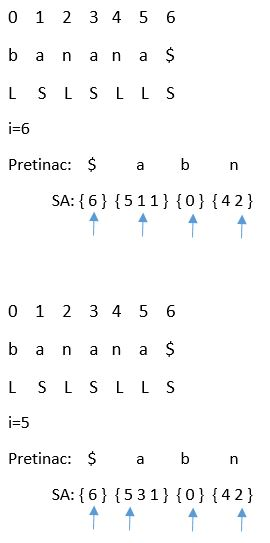
\includegraphics{./pictures/SAISstep3.jpg}
 \caption{Prvi korak u induciranom sortiranju}
 \label{fig:sais3}
\end{figure}

S ta tri koraka završen je postupak induciranog sortiranja koji predstavlja središnji dio ovog algoritma za izgradnju sufiksnog polja. Ovim postupkom smo zapravo djelomično sortirali sve LMS-sufikse. Problem nam predstavljaju LMS-sufiksi koji su jednaki, jer njih na ovaj način ne možemo sortirati. Kako bi sortirali LMS-sufikse moramo još pogledati znakove koji dolaze iza tog LMS-sufiksa. Definirajmo prvo što znaći da su dva LMS-sufiksa jednaka. Dva LMS-sufiksa su jednaka aku su jednake duljine, ako na istim pozicijam imaju jednake znakove i dodatno ako su znakovi na istim pozicijama u oba niza istog tipa (s-znak ili l-znak). Kako bi odredili njihov poredak moramo vidjeti koji LMS-sufiksi slijedi nakon tih LMS-sufiksa. To veoma lako možemo napraviti na način da svakom sufiksu pridjelimo neku leksičku vrijednost, odnosno neki broj. LMS-sufiksi koji su manji dobit će manju leksičku vrijednost, oni koji su veći dobit će veću leksičku vrijednost, dok će jednaki LMS-sufiksi dobiti jednake leksičke vrijednosti. Na taj način smo originalni niz zamjenili kompaktnijim nizom gdje je svaki LMS-sufiks predočen svojom leksičkom vrijednošću. Sada možemo ponoviti cijeli algoritam i na isti način kao i za originalni niz (jer i znakovi su zapravo predstavljeni brojevima, tako da to ništa ne mijenja na stvari) i tako nastavljamo dok ne uspijemo odrediti poredak svih LMS-sufiksa. Kada je on određen, indukcijom lako dobijemo poredak svih L-sufiksa i S-sufiksa te je time postupak računanja sufiksnog polja dovršen.

Sada kada smo pogledali sve korake algoritma zasebno, rezimirajmo cjelokupni algoritam još jednom. U prvom koraku je potrebno odrediti tipove svih znakova (da li je znak l-znak ili s-znak), kao i koji su znakovi LMS-znakovi. Drugi korak algoritma je provođenje induciranog sortiranja nad ulaznim nizom. Time smo dobili međusobno sortirane LMS-nizove, no bitno je za zapamtiti da su sortirani samo oni koji su međusobno u potpunosti različiti. Ukoliko je dva ili više LMS-niza u potpunosti jednako (po jednakosti definiranoj ranije), onda ovim korakom nije jednoznačno određeno koji je od tih LMS-nizova nizova manji a koji veći. Kako bi odredili poredak LMS-nizova potrebno ih je ponovo sortirati, i to radimo tako da sve LMS-nizove zamijenimo leksikografskim znakovima po principu da LMS-nizovi koji se u sortiranom poretku pojavljuju ranije dobe manje leksikografkse znakove, jednakim LMS-nizovima pridjele se jednaki leksikografksi znakovi i onim LMS-znakovima koji se pojavljuju kasnije pridjele veće leksičke vrijednosti. Time smo stvorili novi, reducirani, problem koji možemo riješiti istim postupkom kao i originalni problem. Kada je riješen ovaj reducirani problem, jednoznačno nam je određen poredak LMS-nizova, i sada ukoliko provedemo ponovno inducirano sortiranje, dobit ćemo sufiksno polje.


Kao što vidimo radi se o vrlo jednostavnom, konciznom i elegantnom algoritmu koji u linearnom vremenu može izgraditi sufiksno polje. Teoretski, memorijsko zauzeće algoritma je $O(5n)$, no u implementaciji ono je obično nešto veće zbog dodatnih struktura koje su potrebne za rad algoritma (primjerice polje koje sadrži tipove svih znakova kako se ono ne bi moralo ponovo određivati u pojedinim koracima algoritma). Možda se kao jedna zamjerka algoritma može učiniti to što je potrebno raditi rekurzivne pozive tijekom rješavanja problema, no to nije toliki problem koliki se čini jer je obično broj rekurzivnih poziva dosta malen, čak i za veće nizove.


\section{Wavelet stablo}

Wavelet stablo (engl. \textit{wavelet tree}) je podatkovna struktura koja tekstualni niz organizira u hijerarhiju nizova nula i jedinica - \textit{bit-vektora}. Ova struktura omogućuje pronalazak broja pojavljivanja do nekog indeksa u nizu - \textit{ranga} nekog znaka sa složenošću od $O(log n)$, gdje je $n$ veličina abecede danog tekstualnog niza. 
Stablo se izgrađuje rekurzivno, razdijeljujući abecedu u parove podabeceda. Nakon izgradnje stabla, svaki list odgovara jednom znaku abecede, dok ostali unutarnji čvorovi označavaju da li pojedini znak teksta pripada prvoj ili drugoj podabecedi.
Ukoliko se bit-vektori koji izgrađuju stablo pohrane u RRR strukturu (koja je opisana u idućem poglavlju), moguće je da se memorijsko zauzeće smanji s obzirom na originalno stablo koje ne koristi RRR strukturu.


\subsection{Konstruiranje wavelet stabla}

Wavelet stablo pretvara dovedeni niz u balansirano binarno stablo bit-vektora, gdje se dio znakova, koji pripadaju prvoj polovici dane abecede, kodira kao 0, a drugi dio kao 1. Iako se na prvi pogled čini kako ovo unosi nejednoznačnost u dekodiranju sadržaja stabla, to ipak nije tako. Naime, prelaskom u slijedeću razinu, prva polovica abecede iz prethodne razine ponovno se dijeli na dva dijela te se njeni znakovi ponovo kodiraju kao 0 ili 1. Postupak se rekurzivno nastavlja sve dok se abeceda ne sadrži samo dva znaka, koji se tada jednoznačno kodiraju; prvi s 0, a drugi s 1. 
Originalna podjela ulazne abecede koju su predložili Grossi, Grupta i Vitter \cite{wavelet}  abecedu uvijek dijeli na dva jednaka dijela. Podjela abecede koja je implementirana u sklopu ovog projekta razlikuje se od originalne. Naime, kako bi se ujednačila veličina podijeljenih abeceda, a time i memorijsko zauzeće strukture, abecede se dijele na osnovu učestalosti pojavljivanja pojedinog znaka abecede unutar ulaznog niza. U ovoj implementaciji, abeceda se dijeli na prvom znaku čiji broj pojavljivanja u ulaznog nizu, zbrojen s ukupnim brojem pojavljivanja svih znakova koji su u abecedi njegovi prethodnici, veći ili jednak polovici veličine ulaznog niza.
Na slici \ref{usporedba} prikazana je usporedba izgradnje stabla originalnim (gore) i ovdje implementiranim postupkom (dolje). Abeceda ulaznog niza je {a,b,c,d}. Broj pojavljivanja znaka a je 4, znaka b 1, znaka c 5, a znaka d 10 puta. Veličina ulaznog niza iznosi 20. U prvom slučaju, ulazna abeceda dijeli se na podabecede {a,b} i {c,d}, dok se u drugom slučaju abeceda dijeli na {a,b,c} i {d}. Razlog tomu je što je zbroj broja pojavljivanja znakova a, b i c jednak polovici veličine ulaznog niza.
Razlog zašto je ovaj način memorijski efikasniji objašnjen je u idućem poglavlju iz razloga što ovisi o RRR strukturi koja pohranjuje bit-vektore stabla.

\begin{figure}[H]
\centering
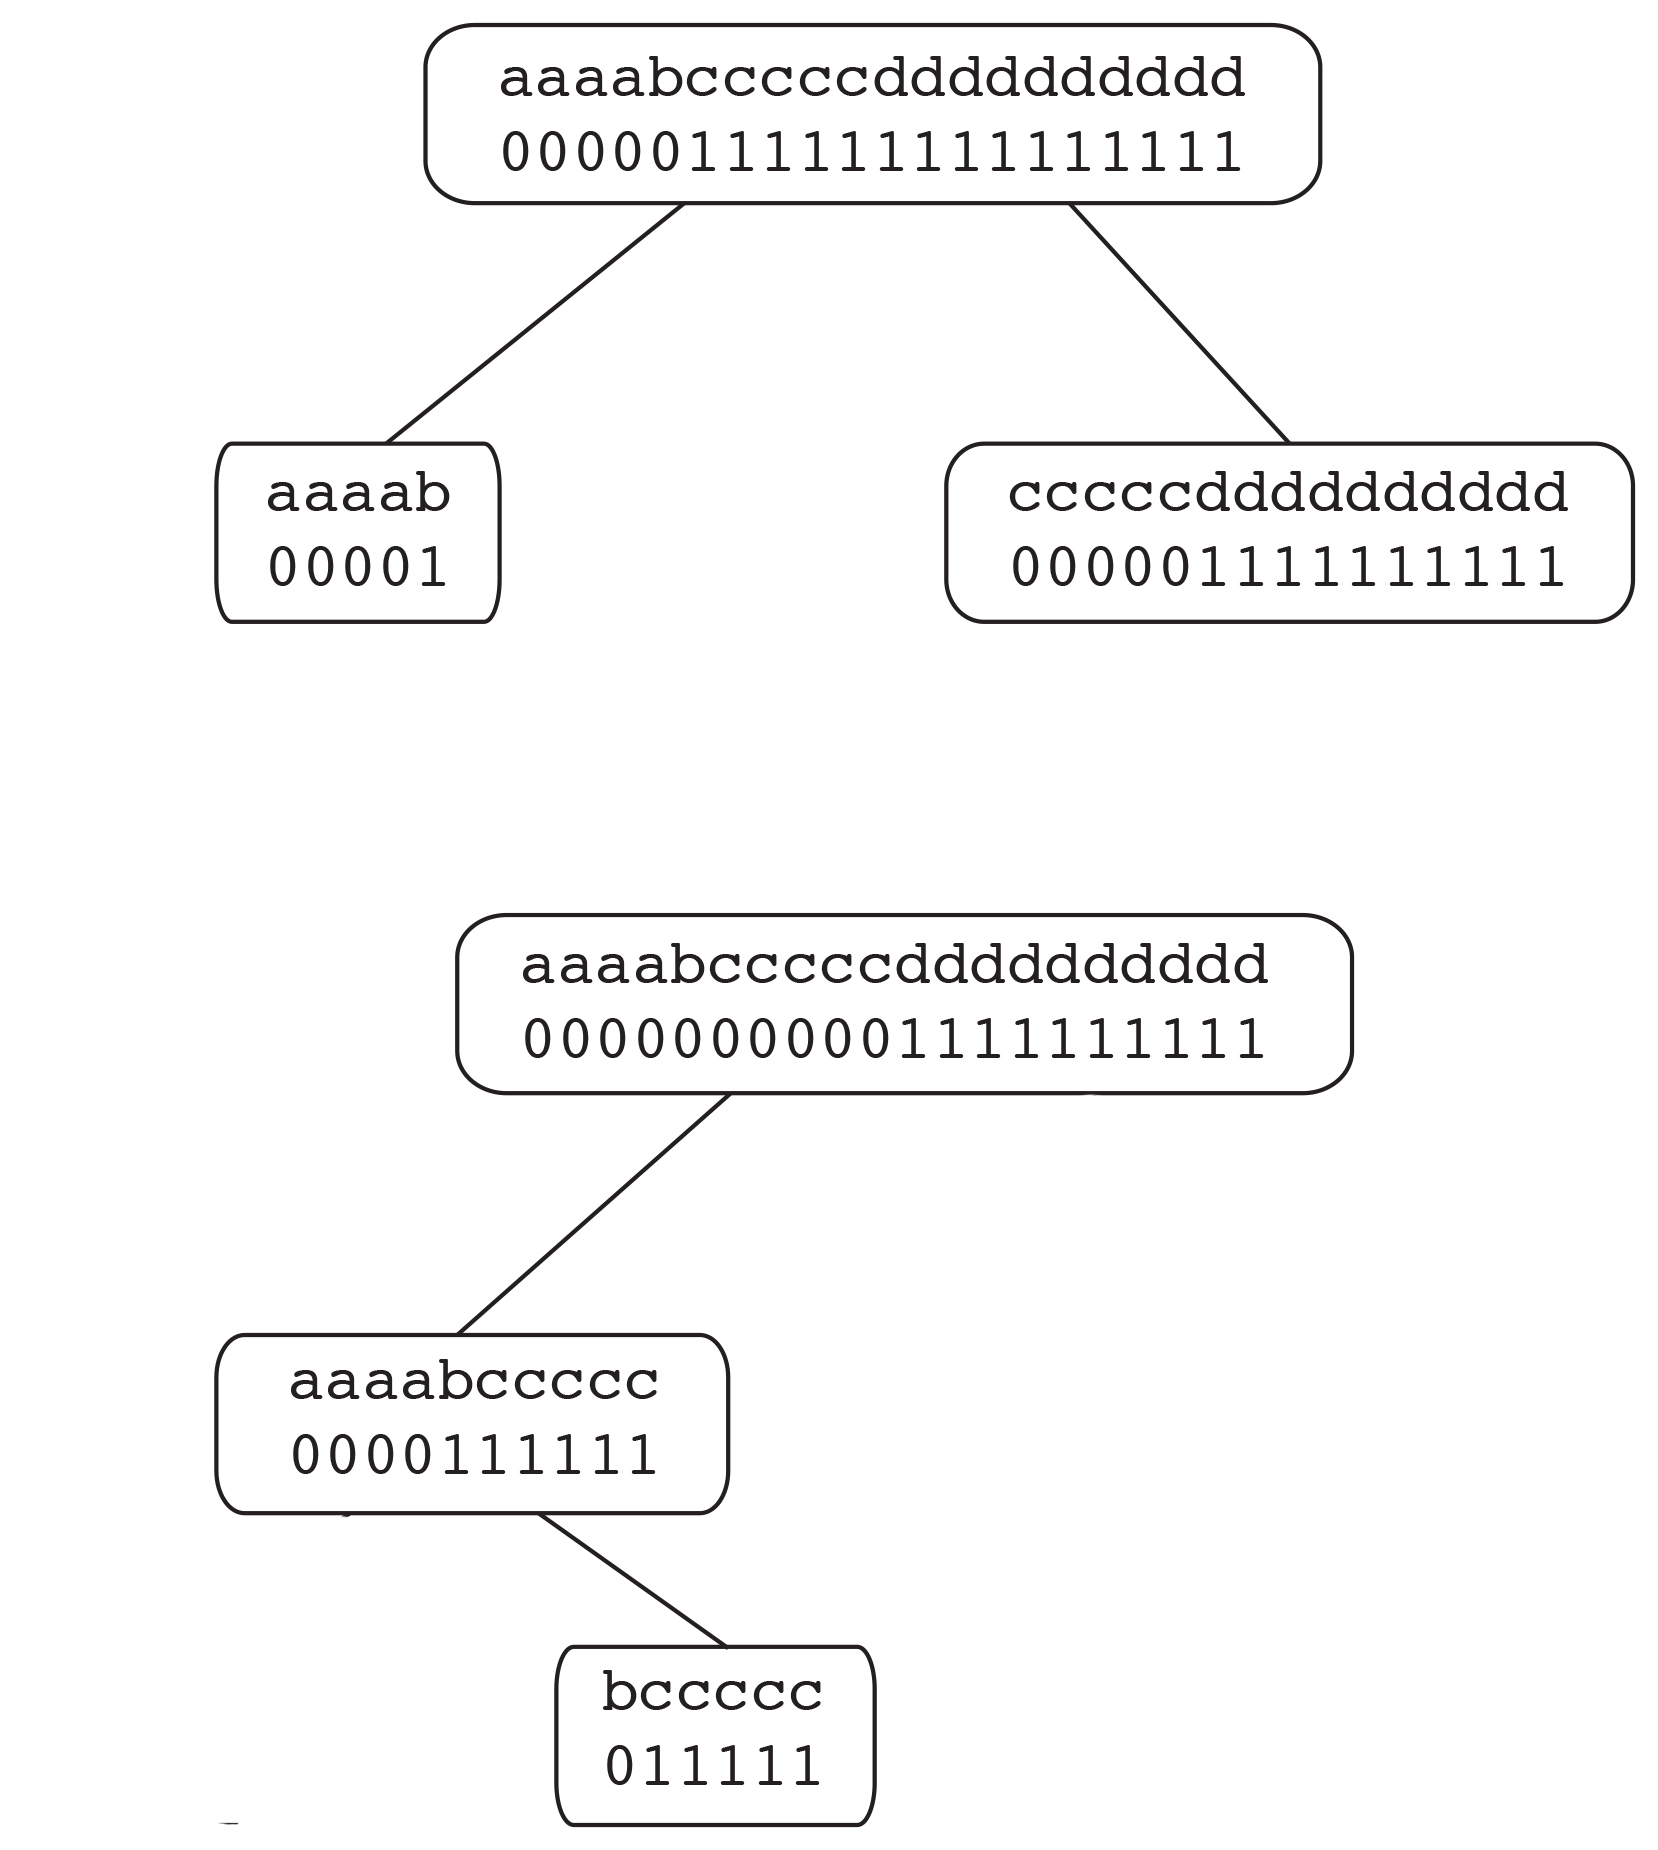
\includegraphics[scale=0.2]{./pictures/Waveletusporedba.jpg}
\caption{Razlika između originalnog i ovdje implementiranog wavelet stabla}\label{usporedba}
\end{figure}



\subsection{Upiti nad wavelet stablom}
Slika \ref{query} prikazuje primjer pronalaska ranga unutar wavelet stabla. Točnije, primjer pronalazi rang znaka c na poziciji 9. U prvom koraku, budući da znamo da je slovo c kodirano s 0, brojimo nule do indeksa 9. Nakon što smo pronašli 7 nula, spuštamo se u slijedeću razinu stabla - u lijevu granu, iz razloga što je znak c kodiran s 0. Sada, u ovoj grani, budući da je znak c kodiran s 1, brojimo koliko ima jedinica u prvih 7 znakova. Važno je primjetiti kako u ovom koraku ustvari idemo do indeksa 6, a ne 7. Nakon što su pronađene 4 jedinice, spuštamo se u iduću razinu, u desnu granu, te brojimo jedinice do četvrtog znaka (indeks 3). U ovoj razini, ujedno i posljednjoj razini stabla, do četvrtog znaka prebrojavamo 3 jedinice iz čega zaključujemo da je rang znaka c na poziciji 9 jednak 3.

\begin{figure}[H]
\centering
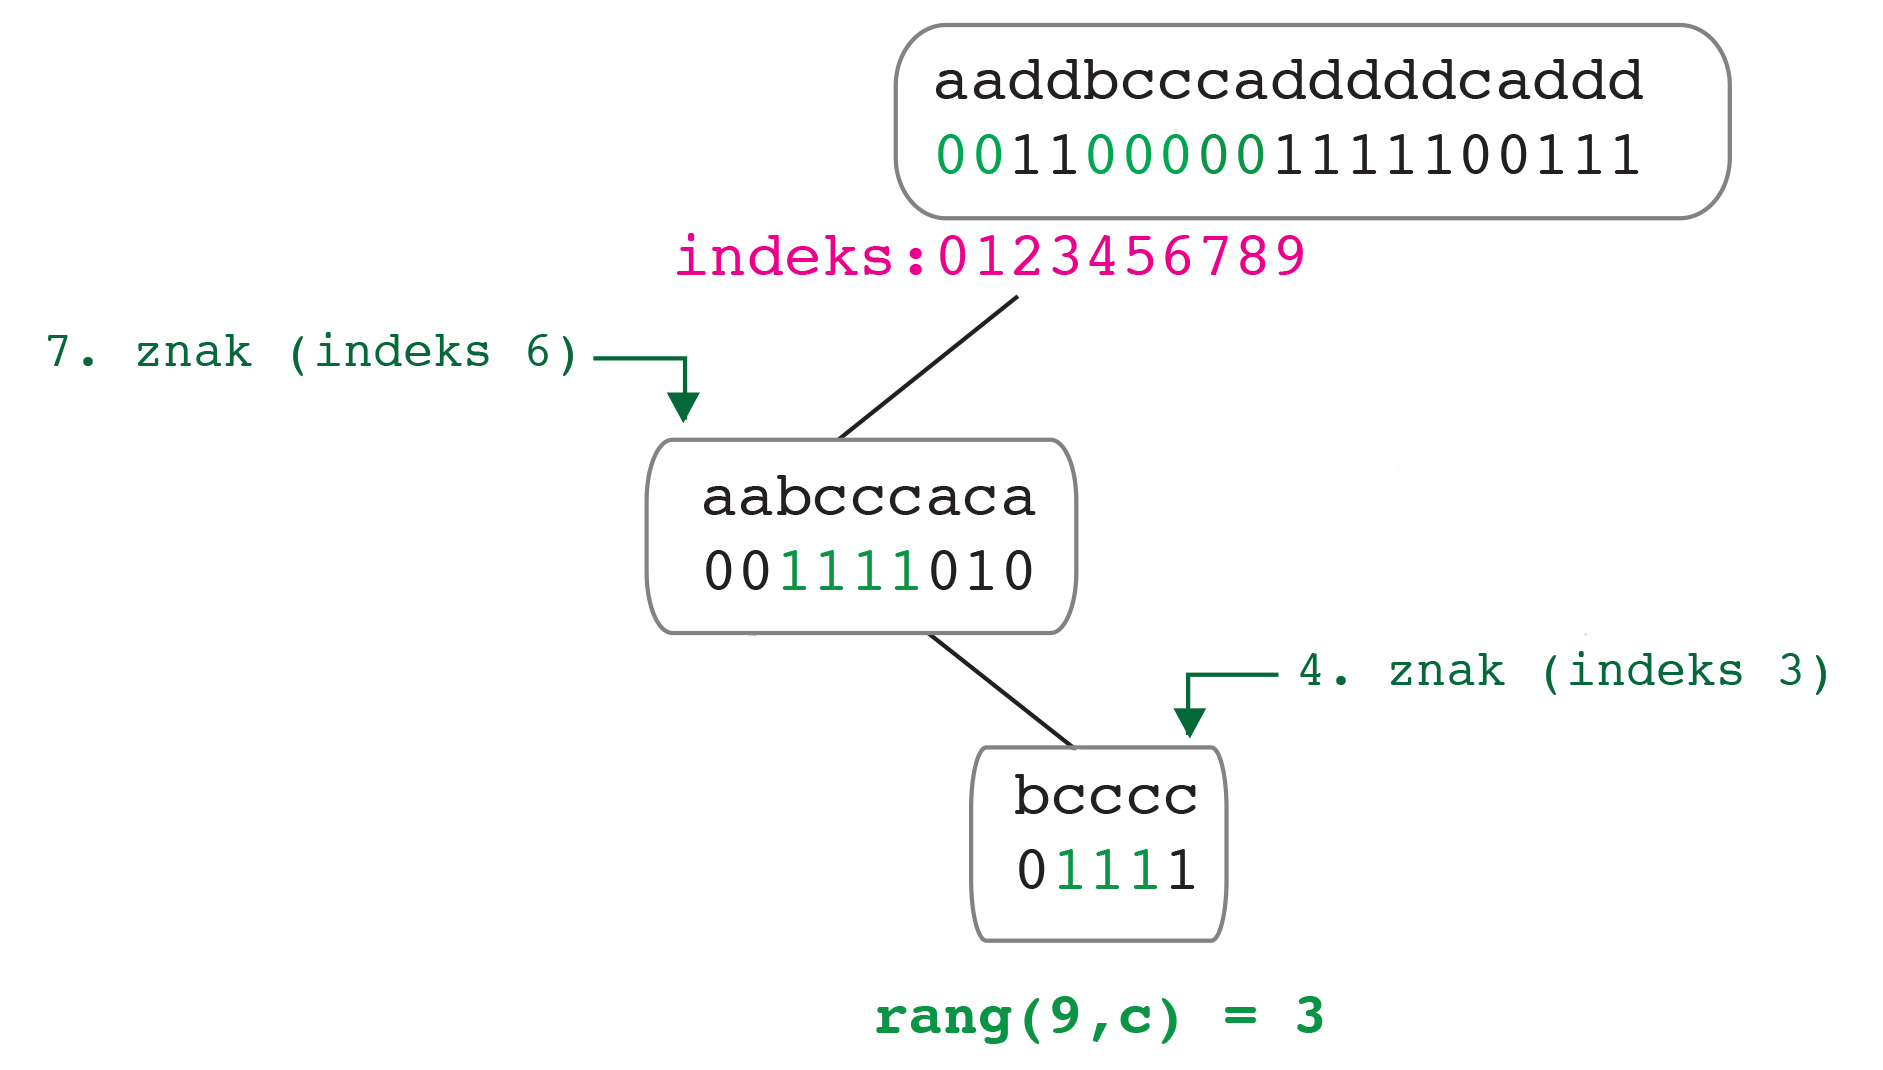
\includegraphics[width=\linewidth]{./pictures/Waveletquery.jpg}
\caption{Razlika između originalnog i ovdje implementiranog wavelet stabla}\label{query}
\end{figure}


\section{RRR struktura}
RRR struktura je struktura koja za dani niz nula i jedinica proizvoljne duljine vraća broj postavljenih jedinica do određene pozicije. Općenito, za dobivanje broja jedinica u nizu nula i jedinica, potrebno je proći kroz cijeli niz i provjeravati svaki element niza. Takvo prebrojavanje niza odvija se u linearnoj vremenskoj složenosti $O(n)$ gdje je $n$ duljina niza. RRR strukturom se ukupan broj jedinica do određene pozicije u nizu može izračunati u konstantnom vremenu $O(1)$. Također, korištenjem RRR strukture se postiže i implicitna kompresija. 

Ideja RRR strukture je da se inicijalno nad nizom konstruiraju blokovi (engl. \textit{buckets}) i nadblokovi (engl. \textit{superbuckets}) u kojima se pohranjuju brojevi jedinica za određene intervale niza. Na taj način se izbjegava pregledavanje cijelog dijela niza u potrazi za brojem jedinica, već je potrebno pregledati samo mali dio niza i određene vrijednosti pohranjene u blokovima i nadbloku. 

RRR struktura implementirana u ovom projektu se djelomično razlikuje od originalne RRR strukture koju su predložili Raman, Raman and Rao \cite{rrr1}. U originalnoj RRR strukturi niz je podijeljen u blokove tako da je svaki blok predstavljen parom (SB,B) te su definirane dodatne tri tablice\cite{rrr2}. Implementacija u ovom projektu je nešto drugačije izvedena, ali je zadržala izračun broja jedinica u nizu u konstantnom vremenu te je opisana u nastavku teksta.

\subsection{Konstruiranje RRR strukture}
U ovoj implementaciji RRR strukture, niz duljine $n$ se dijelio u blokove veličine $l$ i nadblokove veličine $l^2$, a vrijednost $l$ se pritom izračunavala kao logaritam duljine niza, tj. $l=log_2 n$. Stvorena su polja BS i SBS veličina $\lfloor n/l \rfloor$ i $\lfloor n/l^{2} \rfloor$ za pohranjivanje vrijednosti blokova i nadblokova. Za stvaranje RRR strukture potrebno je proći kroz cijeli niz znamenki. Brojač jedinica je inicijalno postavljen na nula i povećava se kada se prolaskom kroz niz naiđe na element koji ima vrijednost 1. Kada se prođe kroz $l$ elemenata niza, vrijednost brojača pohranjuje se u polje BS kao zbroj vrijednosti stvorenih blokova u još neispunjenom nadbloku. To znači da se blokovi u jednom nadploku pune kumulativno. Kada se prođe $l^2$ elemenata niza, vrijednost novog nadbloka jednaka je zbroju vrijednosti prošlog nadbloka (ako postoji) i vrijednosti brojača, odnosno zadnjeg konstruiranog bloka. Nakon izračuna vrijednosti nadbloka brojač se postavlja ponovo na vrijednost nula. Primjer ispunjenih vrijednosti u poljima BS i SBS dan je \ref{rrr1}.

\begin{figure}[H]
\centering
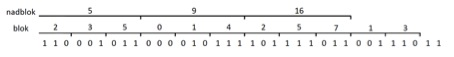
\includegraphics[width=\linewidth]{./pictures/rrr1.png}
\caption{Ispunjene vrijednosti u poljima BS i SBS}\label{rrr1}
\end{figure}

Ukoliko se osvrnemo na primjer wavelet stabla prikazanim u prethodnom poglavlju (\ref{usporedba}), lako možemo izračunati da, ukoliko stablo izgrađujemo originalnim algoritmom, ukupna veličina izgrađenih polja BS i SBS jednaka je 17. Ako se stablo izgradi dijeljenjem abecede na osnovi broja pojavljivanja znakova unutar ulaznog niza, ukupna veličina izgrađenih BS i SBS polja iznosi 14. Već na ovako malom primjeru zamjećuje se poprilična razlika između dobivenih veličina polja BS i SBS.


\subsection{Izračunavanje broja jedinica u nizu}
Broj jedinica u nizu se izračunava kao zbroj vrijednosti zadnjeg popunjenog nadbloka i bloka do zadane pozicije te broja jedinica u ostatku niza koji nije obuhvaćen blokom. Zbog načina punjenja blokova i nadblokova, kod računanja ukupnog broja pojavljivanja jedinica u nizu do određene pozicije potrebno je pripaziti na određene situacije. Ako se tražena pozicija nalazi na mjestu u nizu jednakom $k\cdot l^2$, onda je broj pojavljivanja jedinica u podnizu jednak samo vrijednosti nadbloka, a ako se pozicija nalazi na mjestu u nizu $k\cdot l$, to znači da je vrijednost broja jedinica u podnizu dan ili samo nadblokom (ranije naveden slučaj) ili zbrojem vrijednosti nadbloka i bloka, te nema dijela niza koji nije obuhvaćen blokom/nadblokom za koji treba dodatno provjeravati vrijednosti znamenki. U ostalim slučajevima se vrijednostima zadnjeg popunjenog nadbloka i bloka pridodaje broj jedinica u dijelu niza od zadnjeg popunjenog bloka do pozicije do koje se traži izračun broja pojavljivanja jedinica u podnizu, i to je jedini dio u računanju kada je potrebno slijedno prolaziti kroz elemente niza prebrajajući pojavljivanje jedinica.

U nastavku je opisan postupak izračunavanja broja jedinica za primjer niza prikazanog slikom \ref{rrr2}. Neka se želi izračunati broj pojavljivanja jedinica do pozicije 17. elementa niza (uključujući). Zadnji popunjeni nadblok moguće je pronaći formulom $indNadblok = \linebreak \lfloor pozicija/l^2 \rfloor = \lfloor 17/9 \rfloor = 1$, a zadnji popunjeni blok formulom $indBlok = \lfloor pozicija/l \rfloor = \lfloor 17/3 \rfloor = 5$. Broj pojavljivanja jedinica u ostatku podniza računa se provjeravanjem broja jedinica u dijelu niza od pozicije $indBlok\cdot l+1$ do tražene pozicije (uključujući). U ovom primjeru potrebno je provjeriti pojavljivanje jednica u još dva elementa niza, 16. i 17. elementu, čime se dobiva vrijednost dodatnih jedinica $dodatno$ = 2. Ukupan broj pojavljivanja jedninica u nizu do 17. elementa niza se izračunava kao ukupno  = $SBS(indNadblok) + BS(indBlok) + dodatno = 5 + 1 + 2 = 8$.

\begin{figure}[H]
\centering
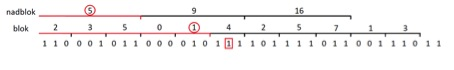
\includegraphics[width=\linewidth]{./pictures/rrr2.png}
\caption{Ispunjene vrijednosti u poljima BS i SBS}\label{rrr2}
\end{figure}
























